Conditional Random Fields are best known for their ability to predict optimal configurations of multiple interdependent variables, which in case of semantic image segmentation are pixels or superpixels. The importance of relations between adjacent superpixels was already presented in the previous chapter, tough only in terms of the pairwise potential. In this chapter a usage of contextual data also in the local potential will be described. The goal of this part of the system is to differentiate objects by their shape. In the dataset for the experiments of this part of the system an object looking like a letter H was introduced. This object is always in the shades of red and is surrounded by greenish superpixels. In order to proof that indeed the shape of the object is recognised, also squares and circles were introduced, which base colour and colours of the surrounding is the same as in case of the letter H. Figure \ref{fig:nonlinear_goal} depicts how those object look. 
\begin{figure}[ht]
    \centering
    \begin{tabular}{ccc}
        \fcolorbox{black}{white}{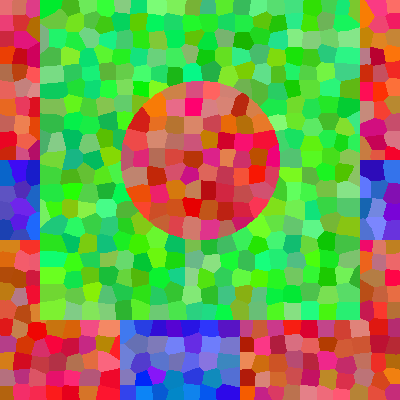
\includegraphics[width = 0.28\textwidth]{nonlinear_intro/circle.png}} &
        \fcolorbox{black}{white}{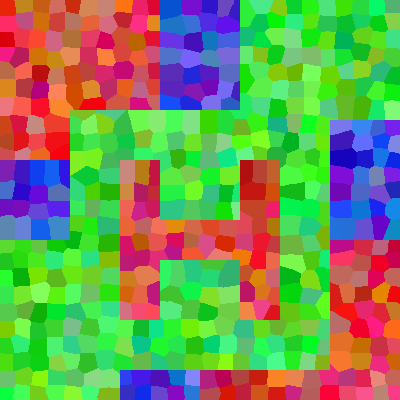
\includegraphics[width = 0.28\textwidth]{nonlinear_intro/letter_h.png}} &
        \fcolorbox{black}{white}{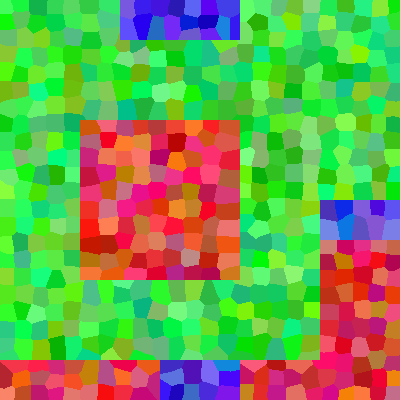
\includegraphics[width = 0.28\textwidth]{nonlinear_intro/square.png}} 
    \end{tabular}
    \caption{Sample images that are to be differentiated basing on their shape.}
    \label{fig:nonlinear_goal}
\end{figure}
Similarly as before label 0 is class for red superpixels, label 1 for green and label 2 for blue, however, this time another class was introduced, denoted as label 3, which is devoted only to the objects with a shape of letter H.

